\newcommand{\QUATROpAmostral}{\num{0.2700}\xspace}
\newcommand{\QUATROn}{200\xspace}
\newcommand{\QUATROy}{\num{54.0000}\xspace}
\newcommand{\QUATROyLinha}{\num{54.5000}\xspace}
\newcommand{\QUATROz}{\num{2.5633}\xspace}
\newcommand{\QUATROpValue}{\num{0.0052}\xspace}
\newcommand{\QUATROesVinte}{\num{0.0000}\xspace}
\newcommand{\QUATROesVinteUm}{\num{0.0248}\xspace}
\newcommand{\QUATROesVinteDois}{\num{0.0491}\xspace}
\newcommand{\QUATROesVinteTres}{\num{0.0731}\xspace}
\newcommand{\QUATROesVinteQuatro}{\num{0.0967}\xspace}
\newcommand{\QUATROesVinteCinco}{\num{0.1199}\xspace}
\newcommand{\QUATROesVinteSeis}{\num{0.1428}\xspace}
\newcommand{\QUATROesVinteSete}{\num{0.1655}\xspace}
\newcommand{\QUATROpVinte}{\num{0.0100}\xspace}
\newcommand{\QUATROpVinteUm}{\num{0.0241}\xspace}
\newcommand{\QUATROpVinteDois}{\num{0.0514}\xspace}
\newcommand{\QUATROpVinteTres}{\num{0.0980}\xspace}
\newcommand{\QUATROpVinteQuatro}{\num{0.1687}\xspace}
\newcommand{\QUATROpVinteCinco}{\num{0.2641}\xspace}
\newcommand{\QUATROpVinteSeis}{\num{0.3797}\xspace}
\newcommand{\QUATROpVinteSete}{\num{0.5057}\xspace}
\newcommand{\QUATROesAmostra}{\num{0.0731}\xspace}
\newcommand{\QUATROtamanhoAmostra}{\num{4055.1080}\xspace}
\newcommand{\QUATROtamanhoAmostraRounded}{4056\xspace}


	Foram retiradas 200 amostras, sem reposição, com tamanhos $n$ = 4, 8, 16, 30
	e 100, dentre os 4986 alunos que possuíam um valor definido para a variável
	\textit{Renda}.  A população possuí média $\mu$ = ${\UMx}$ para a variável
	\textit{Renda}, com desvio padrão $\sigma$ = ${\UMsd}$.  A \autoref{tab:q1}
	apresenta os valores da média e desvio padrão para cada tamanho de amostra
	e seu respectivo valor esperado de desvio padrão ($\frac{\sigma}{\sqrt{n}}$).

	\begin{table}[h]
	\centering
	\caption{Valores da média e desvio padrão das médias amostrais da variável \textit{Renda}.}
	\label{tab:q1}
	\vspace{0.5em}
	\begin{tabular}{l r r r}
		\toprule
		\textbf{\specialcell{c}{Tamanho das \\Amostras}} & \textbf{\specialcell{c}{Média das\\ Médias}} & \textbf{\specialcell{c}{Média dos\\Desvios Padrões}} & \textbf{$\frac{\sigma}{\sqrt{n}}$}\\
		\midrule
		$4$       & ${\UMxQuatro}$   & ${\UMsdQuatro}$   & ${\UMsdeQuatro}$   \\
		$8$       & ${\UMxOito}$   & ${\UMsdOito}$   & ${\UMsdeOito}$   \\
		$16$      & ${\UMxDezesseis}$  & ${\UMsdDezesseis}$  & ${\UMsdeDezesseis}$  \\
		$30$      & ${\UMxTrinta}$  & ${\UMsdTrinta}$  & ${\UMsdeTrinta}$  \\
		$100$     & ${\UMxCem}$ & ${\UMsdCem}$ & ${\UMsdeCem}$ \\
		\bottomrule
	\end{tabular}
	\end{table}

\subsection{Valor Esperado da Média Amostral}

	Na \autoref{tab:q1} é possível observar que a medida que se aumenta o
	tamanho da amostra, a média das médias amostrais fica cada vez mais
	próxima do valor da média populacional, que é de ${\UMx}$.

\subsection{Valor Esperado do Desvio Padrão da Média Amostral}

	Conforme indicado na \autoref{tab:q1}, a média dos desvios padrões
	amostrais ficam mais próximos dos valores de $\frac{\sigma}{\sqrt{n}}$ a
	medida que o tamanho das amostras aumenta.

\subsection{Distribuição Amostral da Média}

	Conforme indicado na Figura \ref{fig:distribuicao-amostral}, a medida
	que o tamanho das amostras aumenta, a distribuição amostral da média se
	torna similar a uma distribuição normal.

\begin{figure}
	\centering
	\begin{subfigure}[b]{0.48\textwidth}
		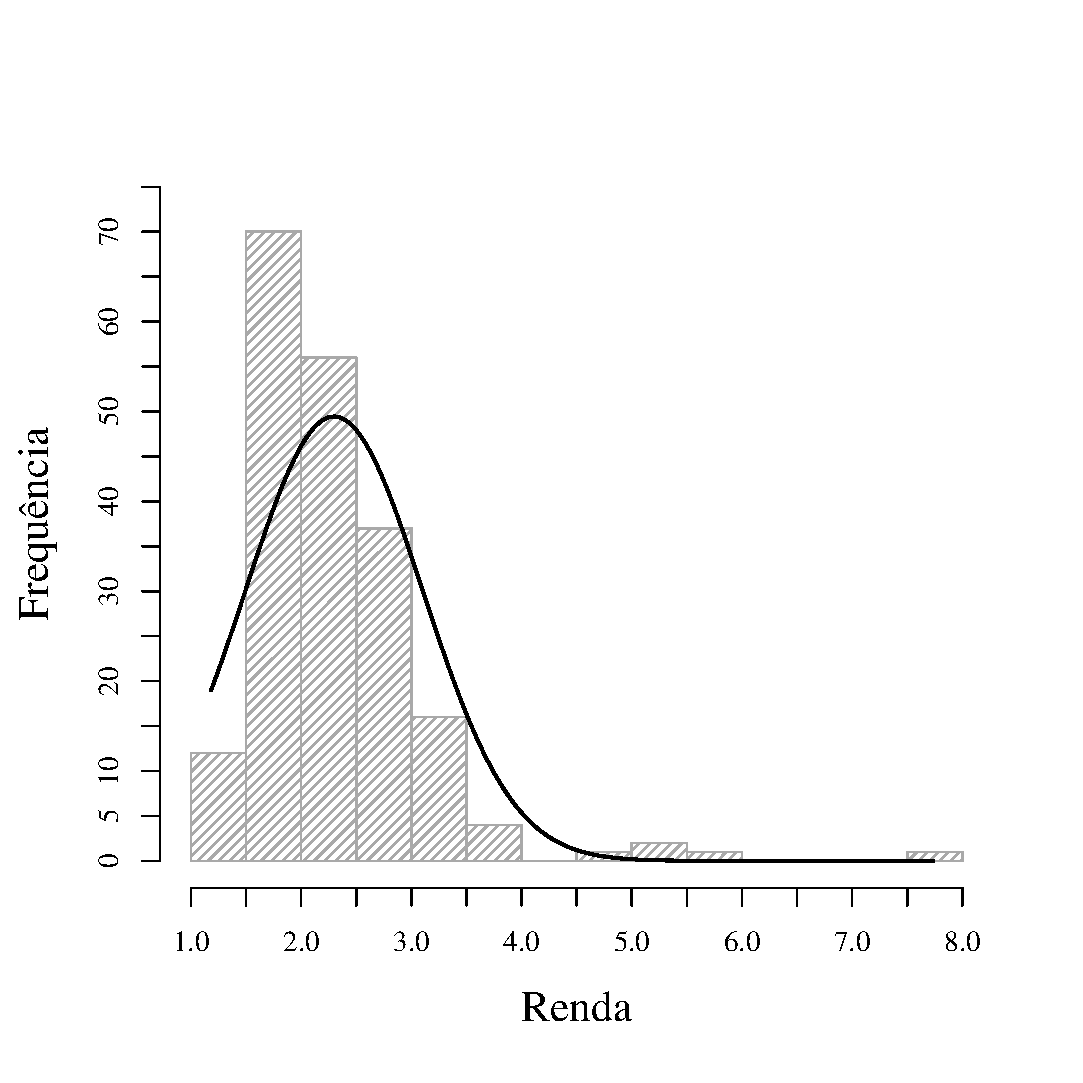
\includegraphics[width=\textwidth]{plots/histogram_renda_n4.eps}
		\caption{}
		\label{fig:m4}
	\end{subfigure}
	~
	\begin{subfigure}[b]{0.48\textwidth}
		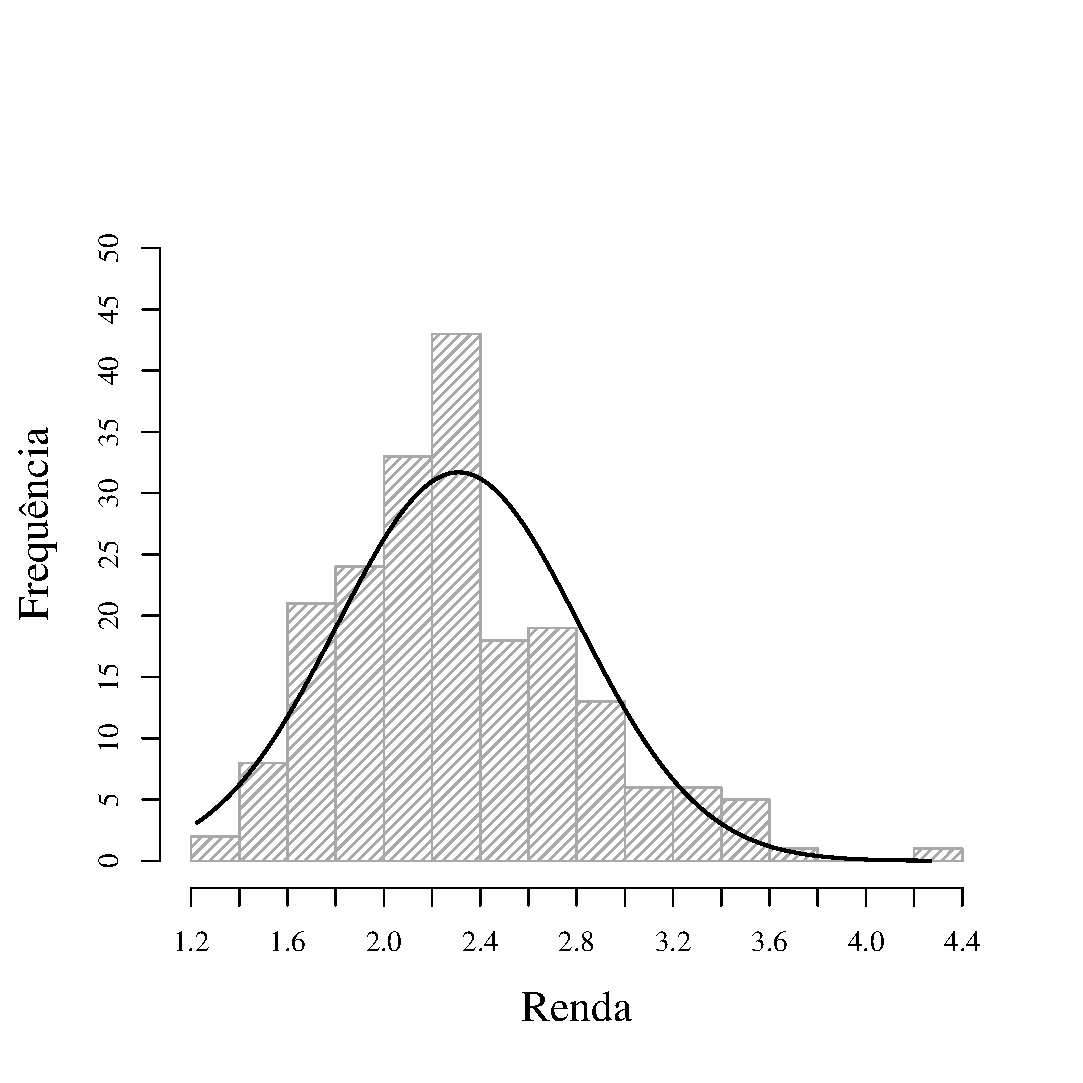
\includegraphics[width=\textwidth]{plots/histogram_renda_n8.eps}
		\caption{}
		\label{fig:m8}
	\end{subfigure}
	\\
	\begin{subfigure}[b]{0.48\textwidth}
		\includegraphics[width=\textwidth]{plots/histogram_renda_n16.eps}
		\caption{}
		\label{fig:m16}
	\end{subfigure}
	~
	\begin{subfigure}[b]{0.48\textwidth}
		\includegraphics[width=\textwidth]{plots/histogram_renda_n30.eps}
		\caption{}
		\label{fig:m30}
	\end{subfigure}
	\\
	\begin{subfigure}[b]{0.48\textwidth}
		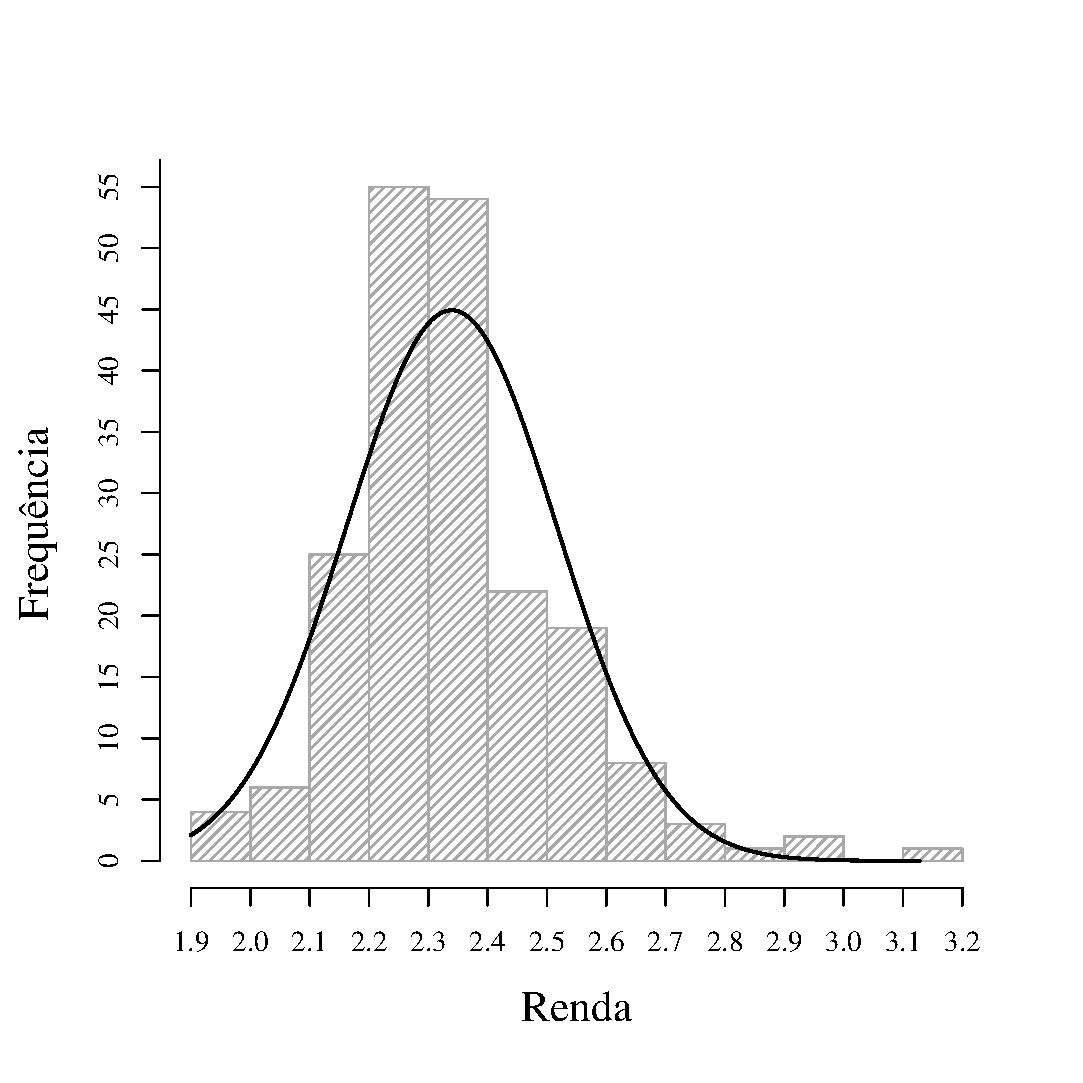
\includegraphics[width=\textwidth]{plots/histogram_renda_n100.eps}
		\caption{}
		\label{fig:m100}
	\end{subfigure}
	\caption{Distribuições amostrais das médias para amostras de tamanho 4(a), 8(b), 16(c), 30(d) e 100(e).}
	\label{fig:distribuicao-amostral}
\end{figure}

\FloatBarrier
